\documentclass{beamer}

\usetheme{avad}

\usepackage[utf8]{inputenc}
\usepackage{amsmath,amssymb}
\usepackage{tikz}

%\graphicspath{%
%{figs/}%
%}



%%%%%%%%%%%%%%%%%%%%%%%%%%%%%%%%%%%%%%%%%%%%%%%%%%%%%%%%%%%%%%%%%%%%%%%%%%%%%%%%
%%%%%%%%%%%%%%%%%%%%%%%%%%%%%%%%%%%%%%%%%%%%%%%%%%%%%%%%%%%%%%%%%%%%%%%%%%%%%%%%
\begin{document}

%%%%%%%%%%%%%%%%%%%%%%%%%%%%%%%%%%%%%%%%%%%%%%%%%%%%%%%%%%%%%%%%%%%%%%%%%%%%%%%%
\title{\centering Open Science in the Two!Ears Project \\ Experiences and Best Practices}
\author{Hagen Wierstorf$\,$\inst{1} \and
        Fiete Winter\inst{2} \and
        \textbf{Sascha Spors}\inst{2}}
        \institute{\inst{1} Centre for Vision, Speech and Signal Processing, University of Surrey\\
           \inst{2} Institute of Communications Engineering, University of Rostock}
\date{26/06/2017}
\maketitle

%%%%%%%%%%%%%%%%%%%%%%%%%%%%%%%%%%%%%%%%%%%%%%%%%%%%%%%%%%%%%%%%%%%%%%%%%%%%%%%%
\begin{frame}{Two!Ears}

    \centering
    \vspace{0.5cm}
    \textbf{Computational framework for modelling active exploratory
    listening that assigns meaning to auditory scenes}

    \vspace{1.0cm}

    \begin{minipage}[b]{0.42\columnwidth}
        \resizebox{\textwidth}{!}{%
            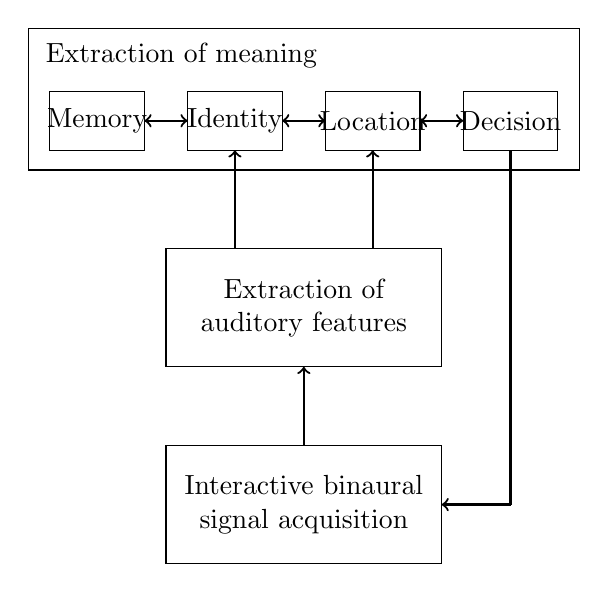
\begin{tikzpicture}
                \draw (-1.75,0) rectangle (1.75,1.5); % binaural simulator
                \node[align=center] at (0,0.75) {Interactive binaural\\ signal acquisition};
                \draw (-1.75,2.5) rectangle (1.75,4); % auditory front-end
                \node[align=center] at (0,3.25) {Extraction of\\ auditory features};
                \draw (-3.5,5) rectangle (3.5,6.8); % blackboard
                \node[right] at (-3.4,6.45) {Extraction of meaning};
                \draw (-3.225,5.25) rectangle (-2.025,6);
                \node at (-2.625,5.625) {\ft Memory};
                \draw (-1.475,5.25) rectangle (-0.275,6);
                \node at (-0.875,5.625) {\ft Identity};
                \draw ( 0.275,5.25) rectangle ( 1.475,6);
                \node at (0.875,5.625) {\ft Location};
                \draw ( 2.025,5.25) rectangle ( 3.225,6);
                \node at (2.625,5.625) {\ft Decision};
                \draw[thick,->] (0,1.5) -- (0,2.5);
                \draw[thick,->] (-0.875,4) -- (-0.875,5.25);
                \draw[thick,->] ( 0.875,4) -- ( 0.875,5.25);
                \draw[thick] (2.625,5.25) -- (2.625,0.75);
                \draw[thick,->] (2.625,0.75) -- (1.75,0.75);
                \draw[thick,<->] (-2.025,5.625) -- (-1.475,5.625);
                \draw[thick,<->] (-0.275,5.625) -- ( 0.275,5.625);
                \draw[thick,<->] ( 1.475,5.625) -- ( 2.025,5.625);
            \end{tikzpicture}
        }
    \end{minipage}
    \hfill
    \begin{minipage}[b]{.54\columnwidth}
        \begin{itemize}
            \item 9 international partners
            \item Test single components
            \item Allow for feedback
            \item Dynamic input signals
        \end{itemize}
        $\Rightarrow$ \textbf{common software} \\
        $\Rightarrow$ \textbf{common data}

        \vspace{1cm}

    \end{minipage}

\end{frame}

%%%%%%%%%%%%%%%%%%%%%%%%%%%%%%%%%%%%%%%%%%%%%%%%%%%%%%%%%%%%%%%%%%%%%%%%%%%%%%%%
\begin{frame}{Open Science}

    Add maybe a slide for an introduction to Open Science

    \begin{itemize}
        \item Introduction
        \item Why it would be a good decision for Two!Ears
    \end{itemize}

\end{frame}

%%%%%%%%%%%%%%%%%%%%%%%%%%%%%%%%%%%%%%%%%%%%%%%%%%%%%%%%%%%%%%%%%%%%%%%%%%%%%%%%
\begin{frame}{Comparison with AMToolbox}

    \vspace{0.3cm}

    Auditory Modeling Toolbox
    \vspace{0.1cm}
    \begin{itemize}
        \item AABBA project started in 2009: \textbf{apply binaural models}
        \item Model source code rarely available
        \item Initiated open collection of models: \\
            {\small\url{http://amtoolbox.sourceforge.net}}
    \end{itemize}

    \vspace{0.6cm}

    Additional required features by Two!Ears
    \vspace{0.1cm}
    \begin{itemize}
        \item Block-based processing
        \item Clear separation in feature extraction and machine learning
        \item Easy combination of different models
        \item Initiated dedicated modeling approach: \\
            {\small\url{http://docs.twoears.eu}}
    \end{itemize}

\end{frame}

%%%%%%%%%%%%%%%%%%%%%%%%%%%%%%%%%%%%%%%%%%%%%%%%%%%%%%%%%%%%%%%%%%%%%%%%%%%%%%%%
\begin{frame}{Two!Ears auditory model}

    \vspace{1cm}

    \begin{minipage}[b]{0.42\columnwidth}
        \resizebox{\textwidth}{!}{%
            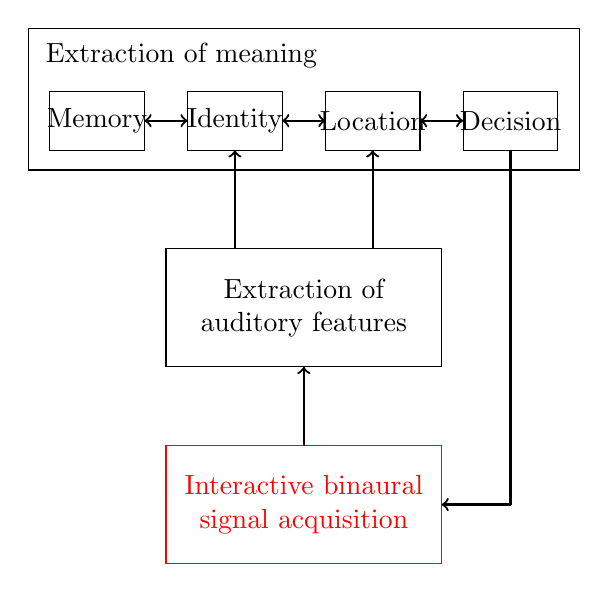
\begin{tikzpicture}
                \draw[color=red] (-1.75,0) rectangle (1.75,1.5); % binaural simulator
                \node[align=center,color=red] at (0,0.75) {Interactive binaural\\ signal acquisition};
                \draw (-1.75,2.5) rectangle (1.75,4); % auditory front-end
                \node[align=center] at (0,3.25) {Extraction of\\ auditory features};
                \draw (-3.5,5) rectangle (3.5,6.8); % blackboard
                \node[right] at (-3.4,6.45) {Extraction of meaning};
                \draw (-3.225,5.25) rectangle (-2.025,6);
                \node at (-2.625,5.625) {\ft Memory};
                \draw (-1.475,5.25) rectangle (-0.275,6);
                \node at (-0.875,5.625) {\ft Identity};
                \draw ( 0.275,5.25) rectangle ( 1.475,6);
                \node at (0.875,5.625) {\ft Location};
                \draw ( 2.025,5.25) rectangle ( 3.225,6);
                \node at (2.625,5.625) {\ft Decision};
                \draw[thick,->] (0,1.5) -- (0,2.5);
                \draw[thick,->] (-0.875,4) -- (-0.875,5.25);
                \draw[thick,->] ( 0.875,4) -- ( 0.875,5.25);
                \draw[thick] (2.625,5.25) -- (2.625,0.75);
                \draw[thick,->] (2.625,0.75) -- (1.75,0.75);
                \draw[thick,<->] (-2.025,5.625) -- (-1.475,5.625);
                \draw[thick,<->] (-0.275,5.625) -- ( 0.275,5.625);
                \draw[thick,<->] ( 1.475,5.625) -- ( 2.025,5.625);
            \end{tikzpicture}
        }
    \end{minipage}
    \hfill
    \begin{minipage}[b]{0.56\columnwidth}

        \centering
        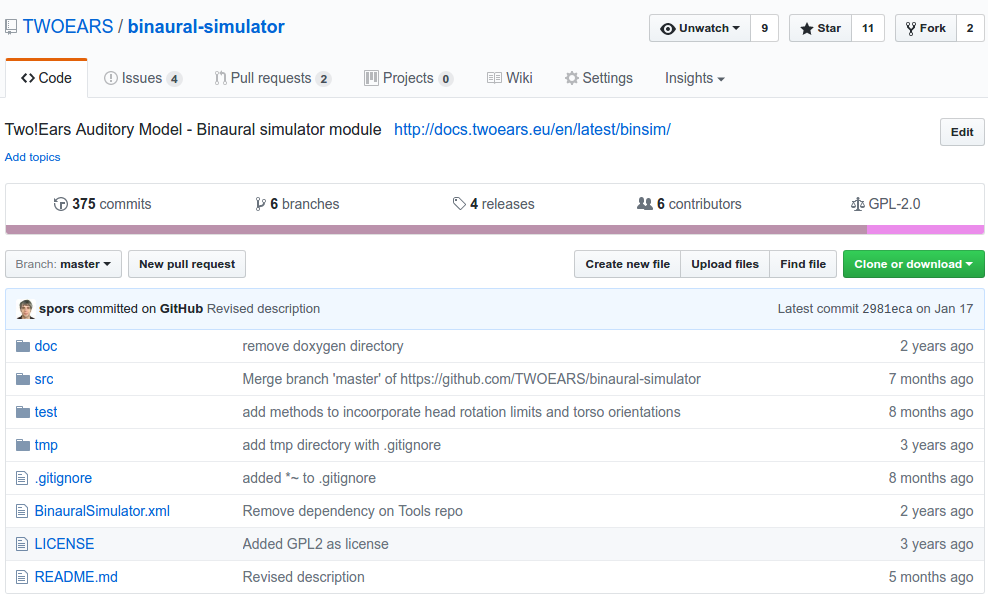
\includegraphics[width=.9\textwidth]{fig/binaural-simulator}

        \begin{itemize}
            \item Standalone ready
            \item Defined interface to other modules
        \end{itemize}

    \end{minipage}

\end{frame}

%%%%%%%%%%%%%%%%%%%%%%%%%%%%%%%%%%%%%%%%%%%%%%%%%%%%%%%%%%%%%%%%%%%%%%%%%%%%%%%%
\begin{frame}{Two!Ears auditory model}

    \vspace{1cm}

    \begin{minipage}[b]{0.42\columnwidth}
        \resizebox{\textwidth}{!}{%
            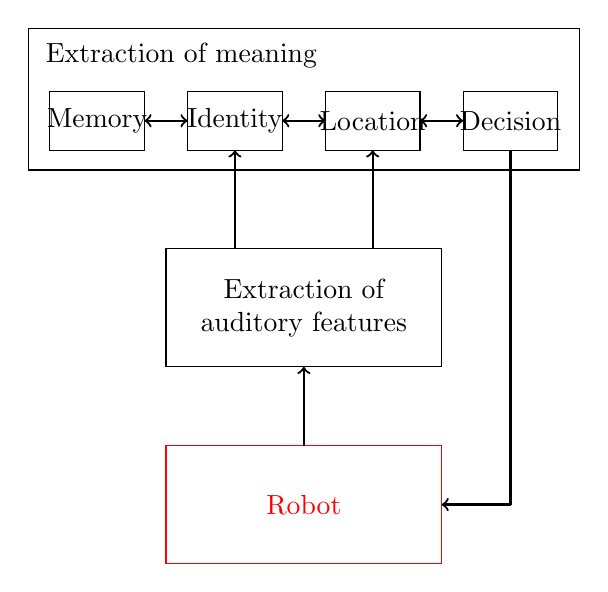
\begin{tikzpicture}
                \draw[color=red] (-1.75,0) rectangle (1.75,1.5); % binaural simulator
                \node[align=center,color=red] at (0,0.75) {Robot};
                \draw (-1.75,2.5) rectangle (1.75,4); % auditory front-end
                \node[align=center] at (0,3.25) {Extraction of\\ auditory features};
                \draw (-3.5,5) rectangle (3.5,6.8); % blackboard
                \node[right] at (-3.4,6.45) {Extraction of meaning};
                \draw (-3.225,5.25) rectangle (-2.025,6);
                \node at (-2.625,5.625) {\ft Memory};
                \draw (-1.475,5.25) rectangle (-0.275,6);
                \node at (-0.875,5.625) {\ft Identity};
                \draw ( 0.275,5.25) rectangle ( 1.475,6);
                \node at (0.875,5.625) {\ft Location};
                \draw ( 2.025,5.25) rectangle ( 3.225,6);
                \node at (2.625,5.625) {\ft Decision};
                \draw[thick,->] (0,1.5) -- (0,2.5);
                \draw[thick,->] (-0.875,4) -- (-0.875,5.25);
                \draw[thick,->] ( 0.875,4) -- ( 0.875,5.25);
                \draw[thick] (2.625,5.25) -- (2.625,0.75);
                \draw[thick,->] (2.625,0.75) -- (1.75,0.75);
                \draw[thick,<->] (-2.025,5.625) -- (-1.475,5.625);
                \draw[thick,<->] (-0.275,5.625) -- ( 0.275,5.625);
                \draw[thick,<->] ( 1.475,5.625) -- ( 2.025,5.625);
            \end{tikzpicture}
        }
    \end{minipage}
    \hfill
    \begin{minipage}[b]{0.56\columnwidth}

        \centering
        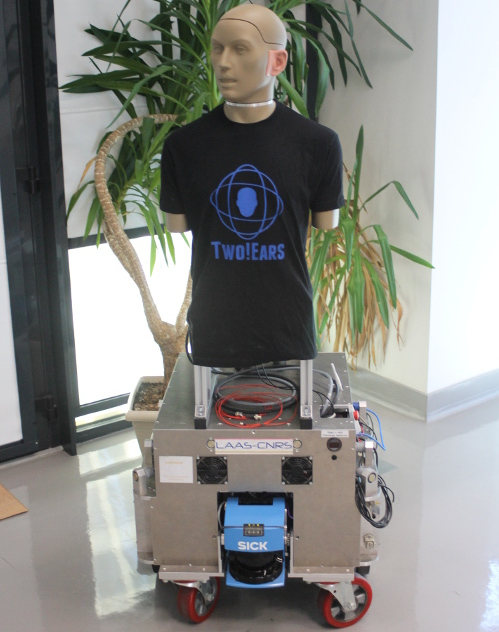
\includegraphics[width=.575\textwidth]{fig/robot}

    \end{minipage}

\end{frame}

%%%%%%%%%%%%%%%%%%%%%%%%%%%%%%%%%%%%%%%%%%%%%%%%%%%%%%%%%%%%%%%%%%%%%%%%%%%%%%%%
\begin{frame}{Two!Ears auditory model}

    \vspace{1cm}

    \begin{minipage}[b]{0.42\columnwidth}
        \resizebox{\textwidth}{!}{%
            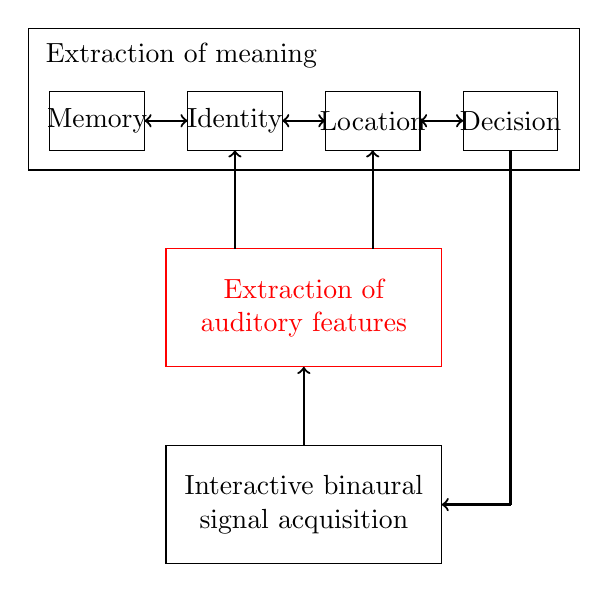
\begin{tikzpicture}
                \draw (-1.75,0) rectangle (1.75,1.5); % binaural simulator
                \node[align=center] at (0,0.75) {Interactive binaural\\ signal acquisition};
                \draw[color=red] (-1.75,2.5) rectangle (1.75,4); % auditory front-end
                \node[align=center,color=red] at (0,3.25) {Extraction of\\ auditory features};
                \draw (-3.5,5) rectangle (3.5,6.8); % blackboard
                \node[right] at (-3.4,6.45) {Extraction of meaning};
                \draw (-3.225,5.25) rectangle (-2.025,6);
                \node at (-2.625,5.625) {\ft Memory};
                \draw (-1.475,5.25) rectangle (-0.275,6);
                \node at (-0.875,5.625) {\ft Identity};
                \draw ( 0.275,5.25) rectangle ( 1.475,6);
                \node at (0.875,5.625) {\ft Location};
                \draw ( 2.025,5.25) rectangle ( 3.225,6);
                \node at (2.625,5.625) {\ft Decision};
                \draw[thick,->] (0,1.5) -- (0,2.5);
                \draw[thick,->] (-0.875,4) -- (-0.875,5.25);
                \draw[thick,->] ( 0.875,4) -- ( 0.875,5.25);
                \draw[thick] (2.625,5.25) -- (2.625,0.75);
                \draw[thick,->] (2.625,0.75) -- (1.75,0.75);
                \draw[thick,<->] (-2.025,5.625) -- (-1.475,5.625);
                \draw[thick,<->] (-0.275,5.625) -- ( 0.275,5.625);
                \draw[thick,<->] ( 1.475,5.625) -- ( 2.025,5.625);
            \end{tikzpicture}
        }
    \end{minipage}
    \hfill
    \begin{minipage}[b]{0.56\columnwidth}

        \centering
        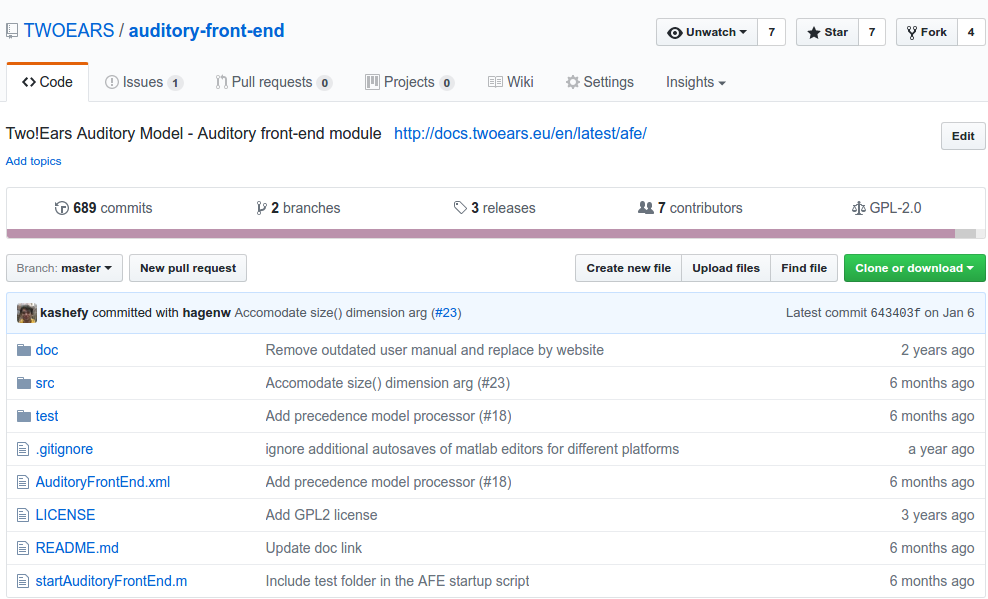
\includegraphics[width=.9\textwidth]{fig/auditory-front-end}

        \begin{itemize}
            \item Standalone ready
            \item Provides auditory features
        \end{itemize}

    \end{minipage}

\end{frame}

%%%%%%%%%%%%%%%%%%%%%%%%%%%%%%%%%%%%%%%%%%%%%%%%%%%%%%%%%%%%%%%%%%%%%%%%%%%%%%%%
\begin{frame}{Two!Ears auditory model}

    \vspace{1cm}

    \begin{minipage}[b]{0.42\columnwidth}
        \resizebox{\textwidth}{!}{%
            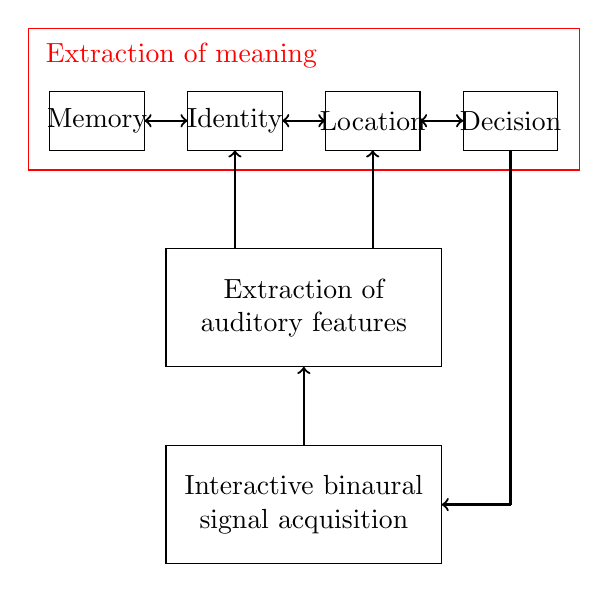
\begin{tikzpicture}
                \draw (-1.75,0) rectangle (1.75,1.5); % binaural simulator
                \node[align=center] at (0,0.75) {Interactive binaural\\ signal acquisition};
                \draw (-1.75,2.5) rectangle (1.75,4); % auditory front-end
                \node[align=center] at (0,3.25) {Extraction of\\ auditory features};
                \draw[color=red] (-3.5,5) rectangle (3.5,6.8); % blackboard
                \node[right,color=red] at (-3.4,6.45) {Extraction of meaning};
                \draw (-3.225,5.25) rectangle (-2.025,6);
                \node at (-2.625,5.625) {\ft Memory};
                \draw (-1.475,5.25) rectangle (-0.275,6);
                \node at (-0.875,5.625) {\ft Identity};
                \draw ( 0.275,5.25) rectangle ( 1.475,6);
                \node at (0.875,5.625) {\ft Location};
                \draw ( 2.025,5.25) rectangle ( 3.225,6);
                \node at (2.625,5.625) {\ft Decision};
                \draw[thick,->] (0,1.5) -- (0,2.5);
                \draw[thick,->] (-0.875,4) -- (-0.875,5.25);
                \draw[thick,->] ( 0.875,4) -- ( 0.875,5.25);
                \draw[thick] (2.625,5.25) -- (2.625,0.75);
                \draw[thick,->] (2.625,0.75) -- (1.75,0.75);
                \draw[thick,<->] (-2.025,5.625) -- (-1.475,5.625);
                \draw[thick,<->] (-0.275,5.625) -- ( 0.275,5.625);
                \draw[thick,<->] ( 1.475,5.625) -- ( 2.025,5.625);
            \end{tikzpicture}
        }
    \end{minipage}
    \hfill
    \begin{minipage}[b]{0.56\columnwidth}

        \centering
        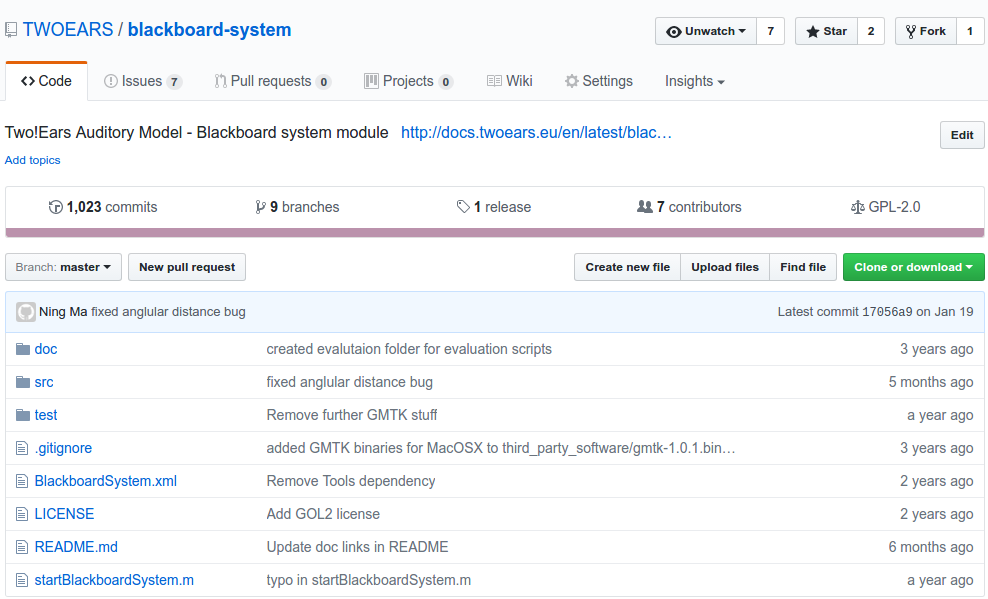
\includegraphics[width=.9\textwidth]{fig/blackboard-system}

        \begin{itemize}
            \item Independent knowledge sources
            \item Needs management
        \end{itemize}

    \end{minipage}

\end{frame}

%%%%%%%%%%%%%%%%%%%%%%%%%%%%%%%%%%%%%%%%%%%%%%%%%%%%%%%%%%%%%%%%%%%%%%%%%%%%%%%%
\begin{frame}{Two!Ears auditory model}

    \vspace{1cm}

    \begin{minipage}[b]{0.42\columnwidth}
        \resizebox{\textwidth}{!}{%
            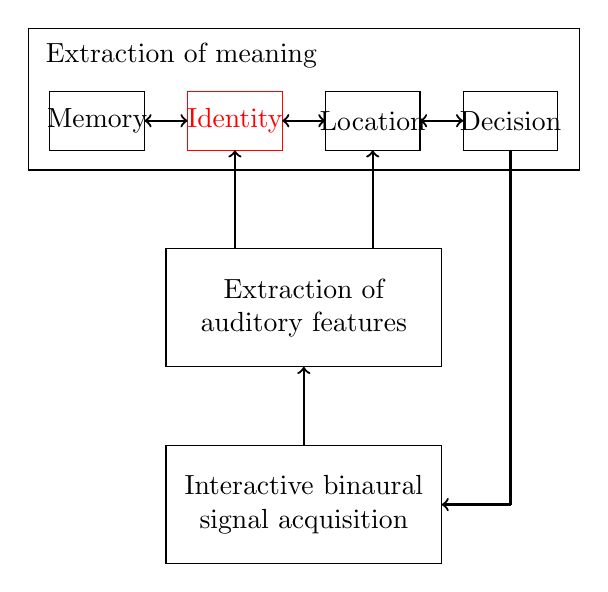
\begin{tikzpicture}
                \draw (-1.75,0) rectangle (1.75,1.5); % binaural simulator
                \node[align=center] at (0,0.75) {Interactive binaural\\ signal acquisition};
                \draw (-1.75,2.5) rectangle (1.75,4); % auditory front-end
                \node[align=center] at (0,3.25) {Extraction of\\ auditory features};
                \draw (-3.5,5) rectangle (3.5,6.8); % blackboard
                \node[right] at (-3.4,6.45) {Extraction of meaning};
                \draw (-3.225,5.25) rectangle (-2.025,6);
                \node at (-2.625,5.625) {\ft Memory};
                \draw[color=red] (-1.475,5.25) rectangle (-0.275,6);
                \node[color=red] at (-0.875,5.625) {\ft Identity};
                \draw ( 0.275,5.25) rectangle ( 1.475,6);
                \node at (0.875,5.625) {\ft Location};
                \draw ( 2.025,5.25) rectangle ( 3.225,6);
                \node at (2.625,5.625) {\ft Decision};
                \draw[thick,->] (0,1.5) -- (0,2.5);
                \draw[thick,->] (-0.875,4) -- (-0.875,5.25);
                \draw[thick,->] ( 0.875,4) -- ( 0.875,5.25);
                \draw[thick] (2.625,5.25) -- (2.625,0.75);
                \draw[thick,->] (2.625,0.75) -- (1.75,0.75);
                \draw[thick,<->] (-2.025,5.625) -- (-1.475,5.625);
                \draw[thick,<->] (-0.275,5.625) -- ( 0.275,5.625);
                \draw[thick,<->] ( 1.475,5.625) -- ( 2.025,5.625);
            \end{tikzpicture}
        }
    \end{minipage}
    \hfill
    \begin{minipage}[b]{0.56\columnwidth}

        \centering
        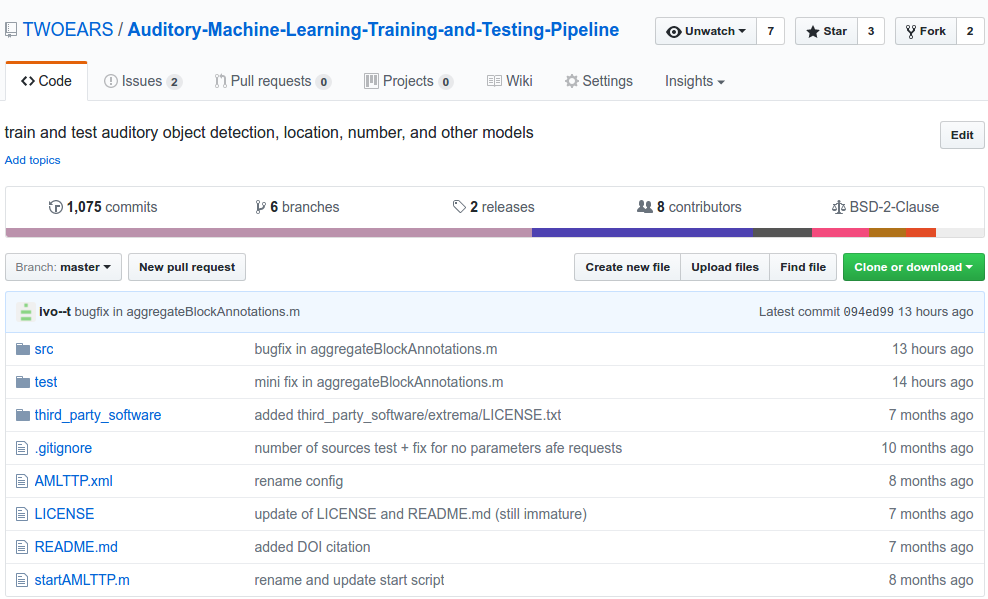
\includegraphics[width=.9\textwidth]{fig/auditory-machine-learning-training}

        \begin{itemize}
            \item Training modules for machine learning
        \end{itemize}

    \end{minipage}

\end{frame}

%%%%%%%%%%%%%%%%%%%%%%%%%%%%%%%%%%%%%%%%%%%%%%%%%%%%%%%%%%%%%%%%%%%%%%%%%%%%%%%%
\begin{frame}{Software depends on data}

    \begin{itemize}
        \item Software development is manageable using revision control, e.g. git
        \item Huge dependency on data:
            \begin{itemize}
                \item HRIR/BRIR measurements for acoustic simulations
                \item Data to train machine learning stages of CASA algorithms
                    (localization, identification, segregation)
                \item Listening test results
            \end{itemize}
        \item Data is collected and changed during the project
        \item All partners need access to it
        \item Not all data can be made publicly available
        \item Need version control for the data as well to ensure everyone is
            using the same version of the data
    \end{itemize}

    How to solve this?

\end{frame}

%%%%%%%%%%%%%%%%%%%%%%%%%%%%%%%%%%%%%%%%%%%%%%%%%%%%%%%%%%%%%%%%%%%%%%%%%%%%%%%%
\begin{frame}{Approaches to data management}

    \begin{itemize}
        \item svn works, but working with branches becomes buggy
        \item git does most probably not work as you will get very soon an out
            of memory error on your server (as git puts everything in working
            memory for packing before transmitting it)
        \item Git Large File Storage (LFS) was released during the project, but
            there was no working implementation to set it up on your own server
        \item There were similar implementations from the community, like
            git-media, git-annex
        \item There have been two commercial providers during the time, but I
            can't find them/remember there name
        \item These two are new ones: \url{https://dataversioncontrol.com},
            \url{http://www.bitkeeper.com/bam.html}
    \end{itemize}

\end{frame}

%%%%%%%%%%%%%%%%%%%%%%%%%%%%%%%%%%%%%%%%%%%%%%%%%%%%%%%%%%%%%%%%%%%%%%%%%%%%%%%%
\begin{frame}{Solution}

    \begin{itemize}
        \item Used a modified version of git-media for internal repo
        \item Used svn for external repo
        \item In both cases you can download single files and subdirectories
        \item git-media hard to install, not everyone in the project was using
            it
        \item git-media still had some bugs
    \end{itemize}

\end{frame}

%%%%%%%%%%%%%%%%%%%%%%%%%%%%%%%%%%%%%%%%%%%%%%%%%%%%%%%%%%%%%%%%%%%%%%%%%%%%%%%%
\begin{frame}{Why we haven't published reproducible paper}

    \begin{itemize}
        \item Awareness was not the same for all members
        \item At the beginning a lot of the software development was happening
            at the partners side and papers were published using that
            (unreleased) software
        \item Should have made a workshop on that topic at the beginning of
            project
        \item Problem remains: it comes with additional time needed (at least at
            the beginning, whereby later on you most probably benefit from it)
    \end{itemize}

\end{frame}

%%%%%%%%%%%%%%%%%%%%%%%%%%%%%%%%%%%%%%%%%%%%%%%%%%%%%%%%%%%%%%%%%%%%%%%%%%%%%%%%
\begin{frame}{Conclusion}

    \begin{itemize}
        \item Extend of software framework to big to be handled only by acoustic
            researchers $\Rightarrow$ loss of time and remaining problems in the
            architecture of the code
        \item Integrate a programmer into your proposal for such projects
    \end{itemize}

\end{frame}


\end{document}
